% !TEX root = ../FundationsDataScience.tex

\chapter{Shannon Theory}
\label{sec-shannon}

%
Shannon theory of information, published in 1948/1949, is made of three parts:
\begin{enumerate}
	\item Sampling: it studies condition under which sampling a continuous function to obtain a discrete vector is invertible. The discrete real values representing the signal are then typically quantized to a finite precision to obtain a set of symbols in a finite alphabet.  
	\item Source coding: it studies optimal ways to represent (code) such a set of symbols as a binary sequence. It leverages the statistical distributions to obtain the most possible compact code.  
	\item Channel coding (not studied here): it studies how to add some redundancy to the coded sequence in order to gain robustness to errors or attacks during transmission (flip of certain bits with some probability). It is often named ``error correcting codes theory''. 
\end{enumerate}
%
The main reference for this chapter is~\cite{mallat2008wavelet}.


%%%%%%%%%%%%%%%%%%%%%%%%%%%%%%%%%%%%%%%%%%%%%%%%%%%%%%%%%%%%%%%%%%%%
%%%%%%%%%%%%%%%%%%%%%%%%%%%%%%%%%%%%%%%%%%%%%%%%%%%%%%%%%%%%%%%%%%%%
%%%%%%%%%%%%%%%%%%%%%%%%%%%%%%%%%%%%%%%%%%%%%%%%%%%%%%%%%%%%%%%%%%%%
\section{Analog vs. Discrete Signals}

To develop numerical tools and analyze their performances, the mathematical modelling is usually done over a continuous setting (so-called ``analog signals''). 
%
Such continuous setting also aims at representing the signal in the physical world, which are inputs to sensors hardwares such as microphone, digital cameras or medical imaging devices. 
%
An analog signal is a 1-D function $f_0 \in \Ldeux([0,1])$ where $[0,1]$ denotes the domain of acquisition, which might for instance be time. An analog image is a 2D function $f_0 \in \Ldeux([0,1]^2)$ where the unit square $[0,1]^2$ is the image domain.

Although these notes are focussed on the processing of sounds and natural images, most of the methods extend to multi-dimensional datasets, which are higher dimensional mappings
\eq{
	f_0 : [0,1]^d \rightarrow [0,1]^s
}
where $d$ is the dimensionality of the input space ($d=1$ for sound and $d=2$ for images) whereas $s$ is the dimensionality of the feature space. For instance, gray scale images corresponds to $(d=2,s=1)$, 
videos to $(d=3, s=1)$, color images to $(d=2, s=3)$ where one has three channels $(R,G,B)$.
One can even consider multi-spectral images where $(d=2, s \gg 3)$ that is made of a large number of channels for different light wavelengths. Figures \ref{fig-examples-1} and \ref{fig-examples-2} show examples of such data.


\myfigure{
	\image{orthobases}{.35}{example-sound}
	\image{orthobases}{.28}{example-image}
	\image{orthobases}{.3}{example-video}
}{%
	Examples of sounds ($d=1$), image ($d=2$) and videos ($d=3$). %	
}{fig-examples-1}

\myfigure{
	\image{orthobases}{.4}{example-color}
	\image{orthobases}{.5}{example-multispectral}
}{%
	Example of color image $s=3$ and multispectral image ($s=32$). %	
}{fig-examples-2}


%%%%%%%%%%%%%%%%%%%%%%%%%%%%%%%%%%%%%%%%%%%
\subsection{Acquisition and Sampling}

Signal acquisition is a low dimensional projection of the continuous signal performed by some hardware device. This is for instance the case for a microphone that acquires 1D samples or a digital camera that acquires 2D pixel samples.
The sampling operation thus corresponds to mapping from the set of continuous functions to a discrete finite dimensional vector with $N$ entries.
\eq{
	f_0 \in \Ldeux([0,1]^d) \mapsto f \in \CC^N
}

\myfigure{
	\image{orthobases}{.4}{discretization-image}
	\image{orthobases}{.5}{discretization-sound}
}{%
	Image and sound discretization. %	
}{fig-discretization}

Figure \ref{fig-discretization} shows examples of discretized signals.

%%%%%%%%%%%%%%%%%%%%%%%%%%%%%%%%%%%%%%%%%%%
\subsection{Linear Translation Invariant Sampler}

A translation invariant sampler performs the acquisition as an inner product between the continuous signal and a constant impulse response $h$ translated at the sample location
\eql{\label{eq-linear-sampling}
	f_n = \int_{-S/2}^{S/2} f_0(x) h(n/N - x) \d x= f_0 \star h(n/N).
}
The precise shape of $h(x)$ depends on the sampling device, and is usually a smooth low pass function that is maximal around $x=0$. The size $S$ of the sampler determines the precision of the sampling device, and is usually of the order of $1/N$ to avoid blurring (if $S$ is too large) or aliasing (if $S$ is too small).

Section \ref{sec-sampling} details how to reverse the sampling operation in the case where the function is smooth.


%%%%%%%%%%%%%%%%%%%%%%%%%%%%%%%%%%%%%%%%%%%%%%%%%%%%%%%%%%%%%%%%%%%%
%%%%%%%%%%%%%%%%%%%%%%%%%%%%%%%%%%%%%%%%%%%%%%%%%%%%%%%%%%%%%%%%%%%%
%%%%%%%%%%%%%%%%%%%%%%%%%%%%%%%%%%%%%%%%%%%%%%%%%%%%%%%%%%%%%%%%%%%%
\section{Shannon Sampling Theorem}
\label{subsec-sampling}

%%%
\paragraph{Reminders about Fourier transform.}

For $f \in L^1(\RR)$, its Fourier transform is defined as
\eql{\label{eq-fourier-transform}
	\foralls \om \in \RR, \quad
	\hat f(\om) \eqdef \int_\RR f(x) e^{-\imath x \om} \d x.
}
One has $\norm{\hat f}^2 = (2\pi)^{-1} \norm{f}^2$, so that $f \mapsto \hat f$ can be extended by continuity to $L^2(\RR)$, which corresponds to computing $\hat f$ as a limit when $T \rightarrow +\infty$ of $\int_{-T}^T f(x) e^{-\imath x \om} \d x$.
%
When $\hat f \in L^1(\RR)$, one can invert the Fourier transform so that
\eql{\label{eq-i-ft}
	f(x) = \frac{1}{2\pi} \int_\RR \hat f(\om) e^{\imath x \om} \d \om, 
}
which shows in particular that $f$ is continuous with vanishing limits at $\pm\infty$. 

The Fourier transform $\Ff : f \mapsto \hat f$ exchanges regularity and decay. For instance, if $f \in C^p(\RR)$ with an integrable Fourier transform, then $\Ff(f^{(p)})(\om) = (\imath \om)^{p} \hat f(\om)$ so that $|\hat f(\om)|=O(1/|\om|^p)$. 
%
Conversely, 
\eql{\label{eq-fourier-regul}
	\int_\RR (1+|\om|)^{p} |\hat f(\om)| \d \om<+\infty
	\qarrq f \in C^p(\RR).
}
For instance, if $\hat f(\om)=O(1/|\om|^{p+2})$, one obtains that $f \in C^p(\RR)$. 

%%%
\paragraph{Reminders about Fourier series.}

We denote $\TT=\RR/2\pi\ZZ$ the torus.
%
A function $f \in L^2(\TT)$ is $2\pi$-periodic, and can be viewed as a function $f \in L^2([0,2\pi])$ (beware that this means that the boundary points are glued together), and its Fourier coefficients are
\eq{
	\foralls n \in \ZZ, \quad 
	\hat f_n \eqdef \frac{1}{2\pi}\int_0^{2\pi} f(x) e^{-\imath x n} \d x.
}
This formula is equivalent to the computation of an inner-product $\hat f_n = \dotp{f}{e_n}$ for the inner-product $\dotp{f}{g} \eqdef \frac{1}{2\pi} \int_\TT f(x) \bar g(x) \d x$. 
%
For this inner product, $(e_n)_n$ is orthonormal and is actually an Hilbert basis, meaning that one reconstructs with the following converging series 
\eql{\label{eq-fourier-series}
	f = \sum_{n \in \ZZ} \dotp{f}{e_n} e_n
}
which means $\norm{f-\sum_{n=-N}^N \dotp{f}{e_n} e_n}_{L^2(\TT)} \rightarrow 0$ for $N \rightarrow +\infty$.
%
The pointwise convergence of~\eqref{eq-fourier-series} at some $x \in \TT$ is ensured if for instance $f$ is differentiable. The series is normally convergent (and hence uniform) if for instance $f$ if of class $C^2$ on $\TT$ sin ce in this case, $\hat f_n = O(1/n^2)$. 
%
If there is a step discontinuities, then there is Gibbs oscillations preventing uniform convergence, but the series still converges to the half of the left and right limit.


%%%
\paragraph{Poisson formula.}

The poisson formula connects the Fourier transform and the Fourier series to sampling and periodization operators.
%
For some function $h(\om)$ defined on $\RR$ (typically the goal is to apply this to $h=\hat f$), its periodization reads
\eql{\label{eq-periodizing}
	h_P(\om) \eqdef \sum_n h(\om-2\pi n).
} 
This formula makes sense if $h \in L^1(\RR)$, and in this case $\norm{h_P}_{L^1(\TT)} \leq \norm{h}_{L^1(\RR)}$ (and there is equality for positive functions). 
%
The Poisson formula, stated in Proposition~\ref{prop-poisson} bellow, corresponds to proving that the following diagram
\eq{
	\begin{array}{rcccl}
						& f(x)  &  \overset{\Ff}{\longrightarrow} &  \hat f(\om) &\\
		\text{sampling}& \downarrow & & \downarrow &\text{periodization} \\
						& (f(n))_n  &  \overset{\text{Fourier serie}}{\longrightarrow} &  \sum_n f(n) e^{-\imath \om n} &\\
	\end{array}
}
is actually commutative.

\begin{prop}[Poisson formula]\label{prop-poisson}
Assume that $\hat f$ has compact support and that $|f(x)| \leq C(1+|x|)^{-3}$ for some $C$. Then one has 
\eql{\label{eq-poisson-formula}
	\foralls \om \in \RR, \quad
	\sum_n f(n) e^{-\imath \om n} = \hat f_P(\om).
}
\end{prop}
\begin{proof}
	Since $\hat f$ is compactly supported, $\hat f_P$ is well defined (it involves only a finite sum) and since $f$ has fast decay, using~\eqref{eq-fourier-regul}, $(\hat f)_P$ is $C^1$. It is thus the sum of its Fourier series
	\eql{\label{eq-poisson-formula}
		(\hat f)_P(\om) = \sum_k c_k e^{\imath k \om},
	} 
	where
	\begin{align*}
		c_k = \frac{1}{2\pi} \int_0^{2\pi} (\hat f)_P(\om) e^{-\imath k \om} \d \om = 
		\frac{1}{2\pi} \int_0^{2\pi} \sum_n \hat f(\om-2\pi n) e^{-\imath k \om}  \d \om .
	\end{align*}
	One has 
	\eq{
		\int_0^{2\pi} \sum_n |\hat f(\om-2\pi n) e^{-\imath k \om}|  \d \om = \int_\RR |\hat f| 
	}
	which is bounded because $\hat f \in L^1(\RR)$ (it has a compact support and is $C^1$), so one can exchange the sum and integral
	\eq{
		c_k = \sum_n \frac{1}{2\pi} \int_0^{2\pi} \hat f(\om-2\pi  n) e^{-\imath k \om}  \d \om
		= \frac{1}{2\pi} \int_{\RR} \hat f(\om) e^{-\imath k \om}  \d \om
		= f(-k)
	}
	where we used the inverse Fourier transform formula~\eqref{eq-i-ft}, which is legit because $\hat f \in L^1(\RR)$.
\end{proof}

%%%
\paragraph{Shannon theorem.}

Shannon sampling theorem state a sufficient condition ensuring that the sampling operator $f \mapsto (f(ns))_n$ is invertible for some sampling step size $s>0$. 
%
It require that $\supp(\hat f) \subset [-\pi/s,\pi/s]$, which, thanks to formula~\eqref{eq-i-ft}, implies that $\hat f$ is $C^\infty$ (in fact it is even analytic). 
%
This theorem was first proved by Wittaker in 1915. It was re-proved and put in perspective in electrical engineering by Nyquist in 1928. It became famous after the paper of Shannon in 1949, which put forward its importance in numerical communications.
%
Figure~\ref{fig-sampling-aliasing} give some insight on how the proof works (left) and more importantly, on what happens when the compact support hypothesis fails (in which case aliasing occurs, see also Figure~\ref{fig-aliasing}). 

\myfigure{
	\image{1-shannon}{.8}{sampling-aliasing}
}{%
	Schematic view for the proof of Theorem~\ref{thm-shannon-sampling}. %	
}{fig-sampling-aliasing}





\begin{thm} \label{thm-shannon-sampling}
	If $|f(x)| \leq C(1+|x|)^{-3}$ for some $C$ and $\supp(\hat f) \subset [-\pi/s,\pi/s]$, then one has
	\eql{\label{eq-shannong-interp}
		\foralls x \in \RR, \quad 
		f(x) = \sum_n f(n s) \sinc(x/s-n) \qwhereq
		\sinc(u) = \frac{\sin(\pi u)}{\pi u}
	}
	with uniform convergence.
\end{thm}

\begin{proof} 
	The change of variable $g \eqdef f(s \cdot)$ results in $\hat g=1/s \hat f(\cdot/s)$, indeed, denoting $z=s x$
	\eq{
		\hat g(\om) = \int f(s x) e^{-\imath \om x} \d x = \frac{1}{s} \int f(z) e^{-\imath (\om/s) z} \d z = \hat f(\om/s)/s, 
	} 
	so that we can restrict our attention to $s=1$.
	%
	The compact support hypothesis implies $\hat f(\om) = 1_{[-\pi,\pi]}(\om) \hat f_P(\om)$.  
	Combining the inversion formula~\eqref{eq-i-ft} with Poisson formula~\eqref{eq-poisson-formula}
	\eq{
		f(x) = \frac{1}{2\pi} \int_{-\pi}^\pi \hat f_P(\om) e^{\imath \om x} \d \om
		= \frac{1}{2\pi} \int_{-\pi}^\pi \sum_n f(n) e^{\imath \om (x-n)} \d \om.
	} 
	Since $f$ has fast decay, $\int_{-\pi}^\pi \sum_n |f(n) e^{\imath \om (x-n)}| \d \om = \sum_n |f(n)| < +\infty$, so that one can exchange summation and integration and obtain
	\eq{
		f(x) = \sum_n f(n)  \frac{1}{2\pi} \int_{-\pi}^\pi e^{\imath \om (x-n)} \d \om = \sum_n f(n) \sinc(x-n).
	}
\end{proof}

\wrapf{1-shannon/sinc}{sinc kernel}
One issue with this reconstruction formula is that it uses a slowly decaying and very oscillating $\sinc$ kernels. In practice, one rarely uses such a kernel for interpolation, and one prefers smoother and more localized kernel. If $\supp(\hat f) \subset [-\pi/s',\pi/s']$ with $s'>s$ (i.e. have a more compact spectrum), one can re-do the proof of the theorem, and one gains some degree of freedom to design the reconstruction kernel, which now can be chosen smoother in Fourier and hence have exponential decay in time. 

%
Spline interpolation are defined by considering $\phi_0=1_{[-1/2,1/2]}$ and $\phi_k = \phi_{k-1} \star \phi_0$ which is a piecewise polynomial of degree $k$ and has bounded derivative of order $k$ (and is of class $C^{k-1}$) with compact support on $[-(k+1)/2,(k+1)/2]$. The reconstruction formula reads $f \approx \tilde f \eqdef \sum_n a_n \phi(\cdot-n)$ where $(a_n)_n$ is computed from the $(f(n))_n$ by solving a linear system (associated to the interpolation property $\tilde f(n)=f(n)$). It is only in the cases $k \in \{0,1\}$ (piecewise constant and affine interpolations) that one has $a_n=f(n)$.
%
In practice, one typically use the cubic spline interpolation, which corresponds to $k=3$.

\texttt{Associated code: test\_sampling.m}

\myfigure{
	\image{1-shannon}{.6}{spline}
}{%
	Cardinal splines as bases functions for interpolation. %	
}{fig-aliasing}



This theorem also explains what happens if $\hat f$ is not supported in $[-\pi/s,\pi/s]$. This leads to aliasing, and high frequency outside this interval leads to low frequency artifacts often referred to as ``aliasing''. If the input signal is not bandlimitted, it is thus very important to pre-filter it (smooth it) before sampling to avoid this phenomena (of course this kills the high frequencies, which are lost), see Figure~\ref{fig-aliasing}. 

\myfigure{
	\image{1-shannon}{.6}{aliasing}
}{%
	Aliasing in the simple case of a sine wave (beware however that this function does not have compact support). %	
}{fig-aliasing}

%%%
\paragraph{Quantization.}

Once the signal have been sampled to obtain a discrete vector, in order to store it and transmit it, it is necessary to quantize the value to some finite precision. 
% 
Section~\ref{sec-transform-coding} presents transform coding, which is an efficient family of compression schemes which operate the quantization over some transformed domain (which correspond to applying a linear transform, usually orthogonal, to the sampled values). This is useful to enhance the performance of the source coding scheme. It is however common to operate directly the quantization over the sampled value. 

Considering for instance a step size $s=1/N$, one samples $(u_n \eqdef f(n/N))_{n=1}^{N} \in \RR^N$ to obtain a finite dimensional data vector of length $N$. Note that dealing with finite data corresponds to restricting the function $f$ to some compact domain (here $[0,1]$) and is contradictory with Shannon sampling theorem, since a function $f$ cannot have a compact support in both space and frequency (so perfect reconstruction never holds when using finite storage).

\wrapf{1-shannon/quantizer}{}

Choosing a quantization step $T$, quantization $v_n = Q_T(u_n) \in \ZZ$ rounds to the nearest multiple of $T$, i.e. 
\eq{
	v = Q_T(u) \quad\Leftrightarrow\quad
	v-\frac{1}{2} \leq u/T < v+\frac{1}{2},
}
see Fig.~\ref{fig-quantizer}. De-quantization is needed to restore a signal, and the best reconstruction (in average or in worse case) is defined by setting $D_T(v) \eqdef T v$. Quantizing and then de-quantizing introduce an error bounded by $T/2$, since $|D_T(Q_T(u))-u| \leq T/2$. 
%
Up to machine precision, quantization is the only source of error (often called ``lossy compression'') in Shannon's standard pipeline.


\myfigure{
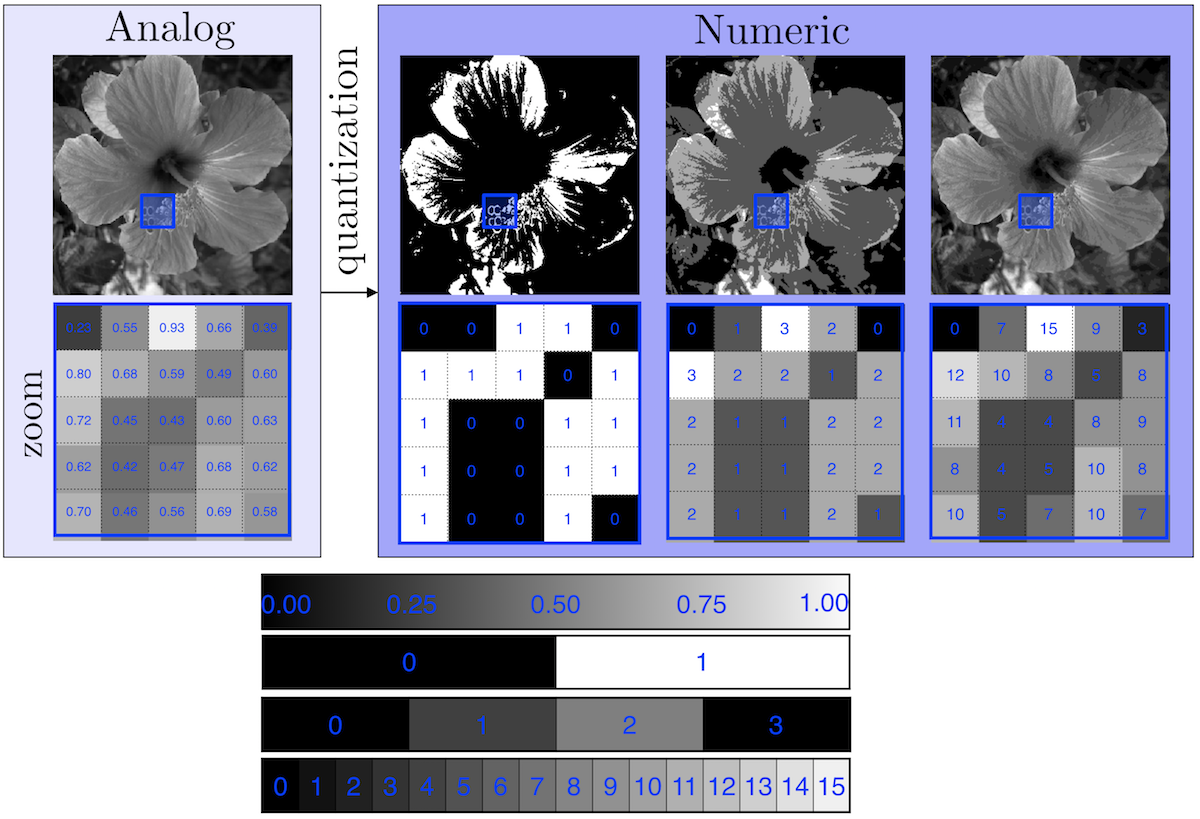
\includegraphics[width=.8\linewidth]{1-shannon/quantize/quantization}
%\tabquatre{
%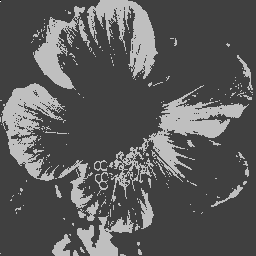
\includegraphics[width=.2\linewidth]{1-shannon/quantize/quantize-2}&
%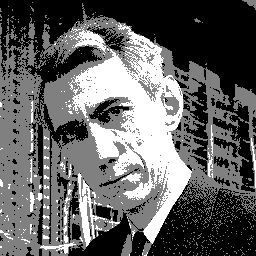
\includegraphics[width=.2\linewidth]{1-shannon/quantize/quantize-3}&
%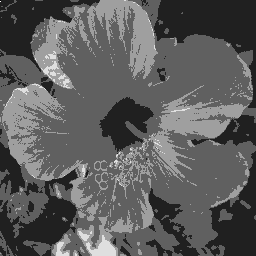
\includegraphics[width=.2\linewidth]{1-shannon/quantize/quantize-4}&
%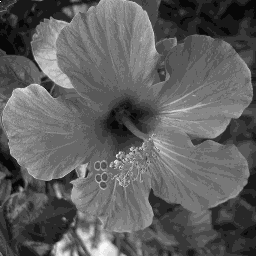
\includegraphics[width=.2\linewidth]{1-shannon/quantize/quantize-16}\\
%$2$ graylevels &
%$3$ graylevels &
%$4$ graylevels &
%$16$ graylevels 
%}
}{Quantizing an image using a decaying $T=1/K$ where $K \in \{2,3,4,16\}$ is the number of graylevels and the original image is normalized so that $0 \leq f_0 < 1$. 
}{fig-section3-quantize}

%%%%%%%%%%%%%%%%%%%%%%%%%%%%%%%%%%%%%%%%%%%%%%%%%%%%%%%%%%%%%%%%%%%%
\section{Shannon Source Coding Theorem}
\label{sec-shannon-source}

\newcommand{\Symb}{s}

%%%
\paragraph{Uniform coding.}

We consider an alphabet $(\Symb_1,\ldots,\Symb_K)$ of $K$ symbols. For instance, if one samples and quantize a bounded signal $0 \leq f_0 < 1$ using a step size $1/K$, then one can consider $\Symb_k=k$ to be integer symbols. For text, these symbols include the letter plus extra punctuation symbols and blank. 
%
It is of course possible to code a sequence of such symbols using a uniform code (e.g. using the base 2 expansion) with $\lceil \log_2(K) \rceil$ bit per symbols.
For instance if $K=4$ and the symbols are $\{0,1,2,3\}$, then the code words are $(c_0=00,c_1=01,c_2=10,c_3=11)$. 

This uniform coding strategy is however extremely inefficient if the symbols are not uniformly distributed (i.e. if some symbols are more frequent than other, which is likely to be the case). We aim at designing better codes.

%%%
\paragraph{Prefix coding.}
 

A code $c_k=c(\Symb_k)$ associate to each symbol $\Symb_k$ a code word $c_k \in \{0,1\}^\NN$ with a varying length $|c_k| \in \NN^*$. 
%
A prefix code $c_k=c(\Symb_k)$ is such that no word $c_k$ is the beginning of another word $c_k'$. This is equivalent to be able to embed the $(c_k)_k$ as leaves of a binary tree $T$, with the code being output of a traversal from root to leaves (with a convention that going to a left (resp. right) child output a 0 (resp. a 1). 
%
We denote $c=\text{Leaves}(T)$ such prefix property. 


\myfigure{
\image{1-shannon}{.35}{tree/prefix-coding}
\qquad
\image{1-shannon}{.35}{tree/tree-example}
}{%
Left: complete tree of all codes of length 3; right: example of prefix code.
}{fig-tree-prefix}

This tree-based representation is useful to decode a binary stream by simply performing tree traversal. One follows the tree, from top to bottom, and outputs a symbol each time a leaf is reached (and then re-start at the top). 


%%
\paragraph{Probabilistic modeling.}

We aim at designing the most possible compact code $c_k$. 
%
We assume at our disposal some probability distribution over this alphabet, which is just an histogram $p=(p_1,\ldots,p_K) \in \RR_+^K$ in the simplex, i.e. $\sum_k p_k=1$. 
%
In practice, this probability is usually the empirical probability of appearance of the symbols $x_k$ in the data to be coded. 

\wrapf{1-shannon/entropie/entropie-fonction}{}

The entropy of such an histogram is 
\eq{
	H(p) \eqdef -\sum_k p_k \log_2(p_k)
}
with the convention $0\log_2(0)=0$. 

Denoting $h(u)=-u \log_2(u)$, $h'(u) \propto -\log(u)-1$, $h''(u) \propto -1/u<0$ so that $H$ is strictly concave. The definition of the entropy extends to continuous density $f(x)$ for $x$ on some measure space with reference measure $\d x$ (e.g. Lebesgue on $\RR^d$) by setting $H(f) \eqdef -\int f(x) \log(f(x)) \d x$. 

\myfigure{
\tabquatre{
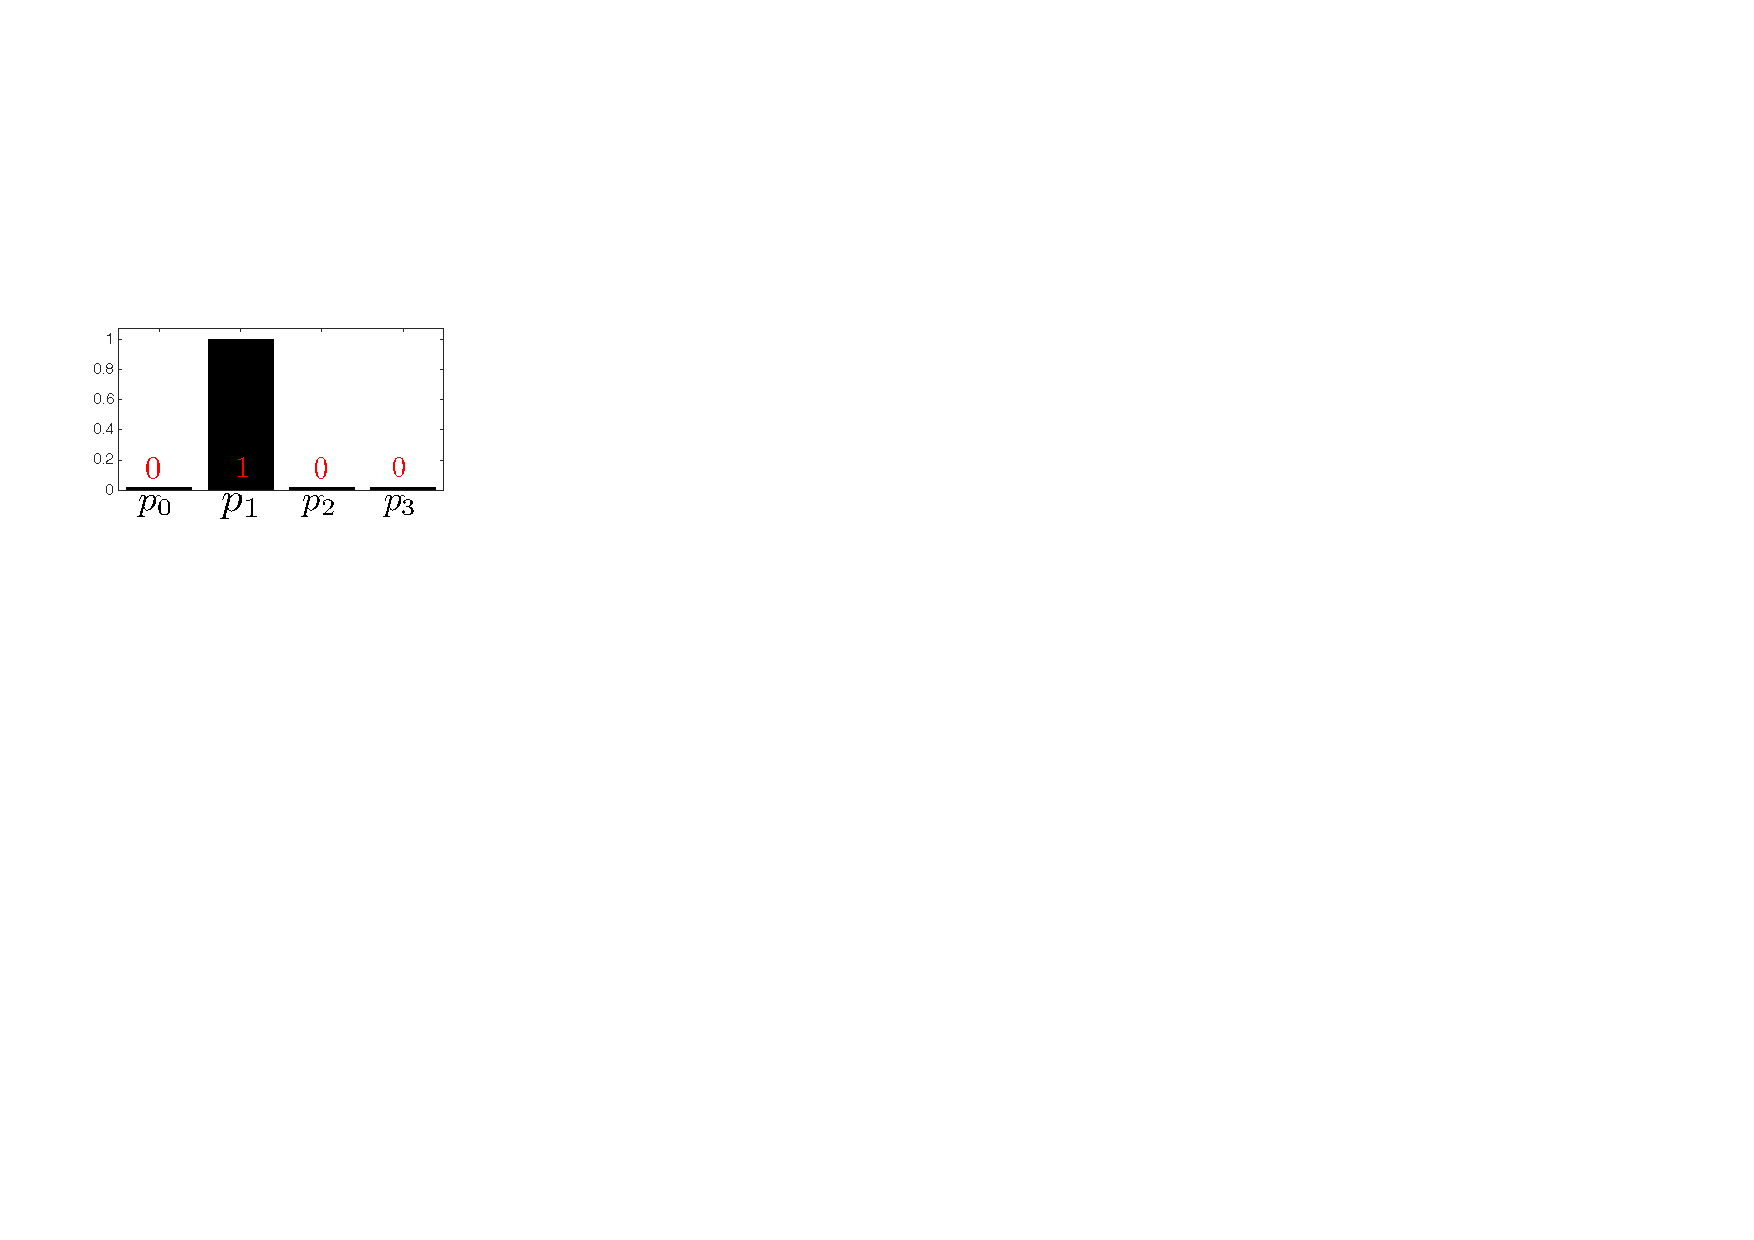
\includegraphics[width=.25\linewidth]{1-shannon/entropie/histo-1}&
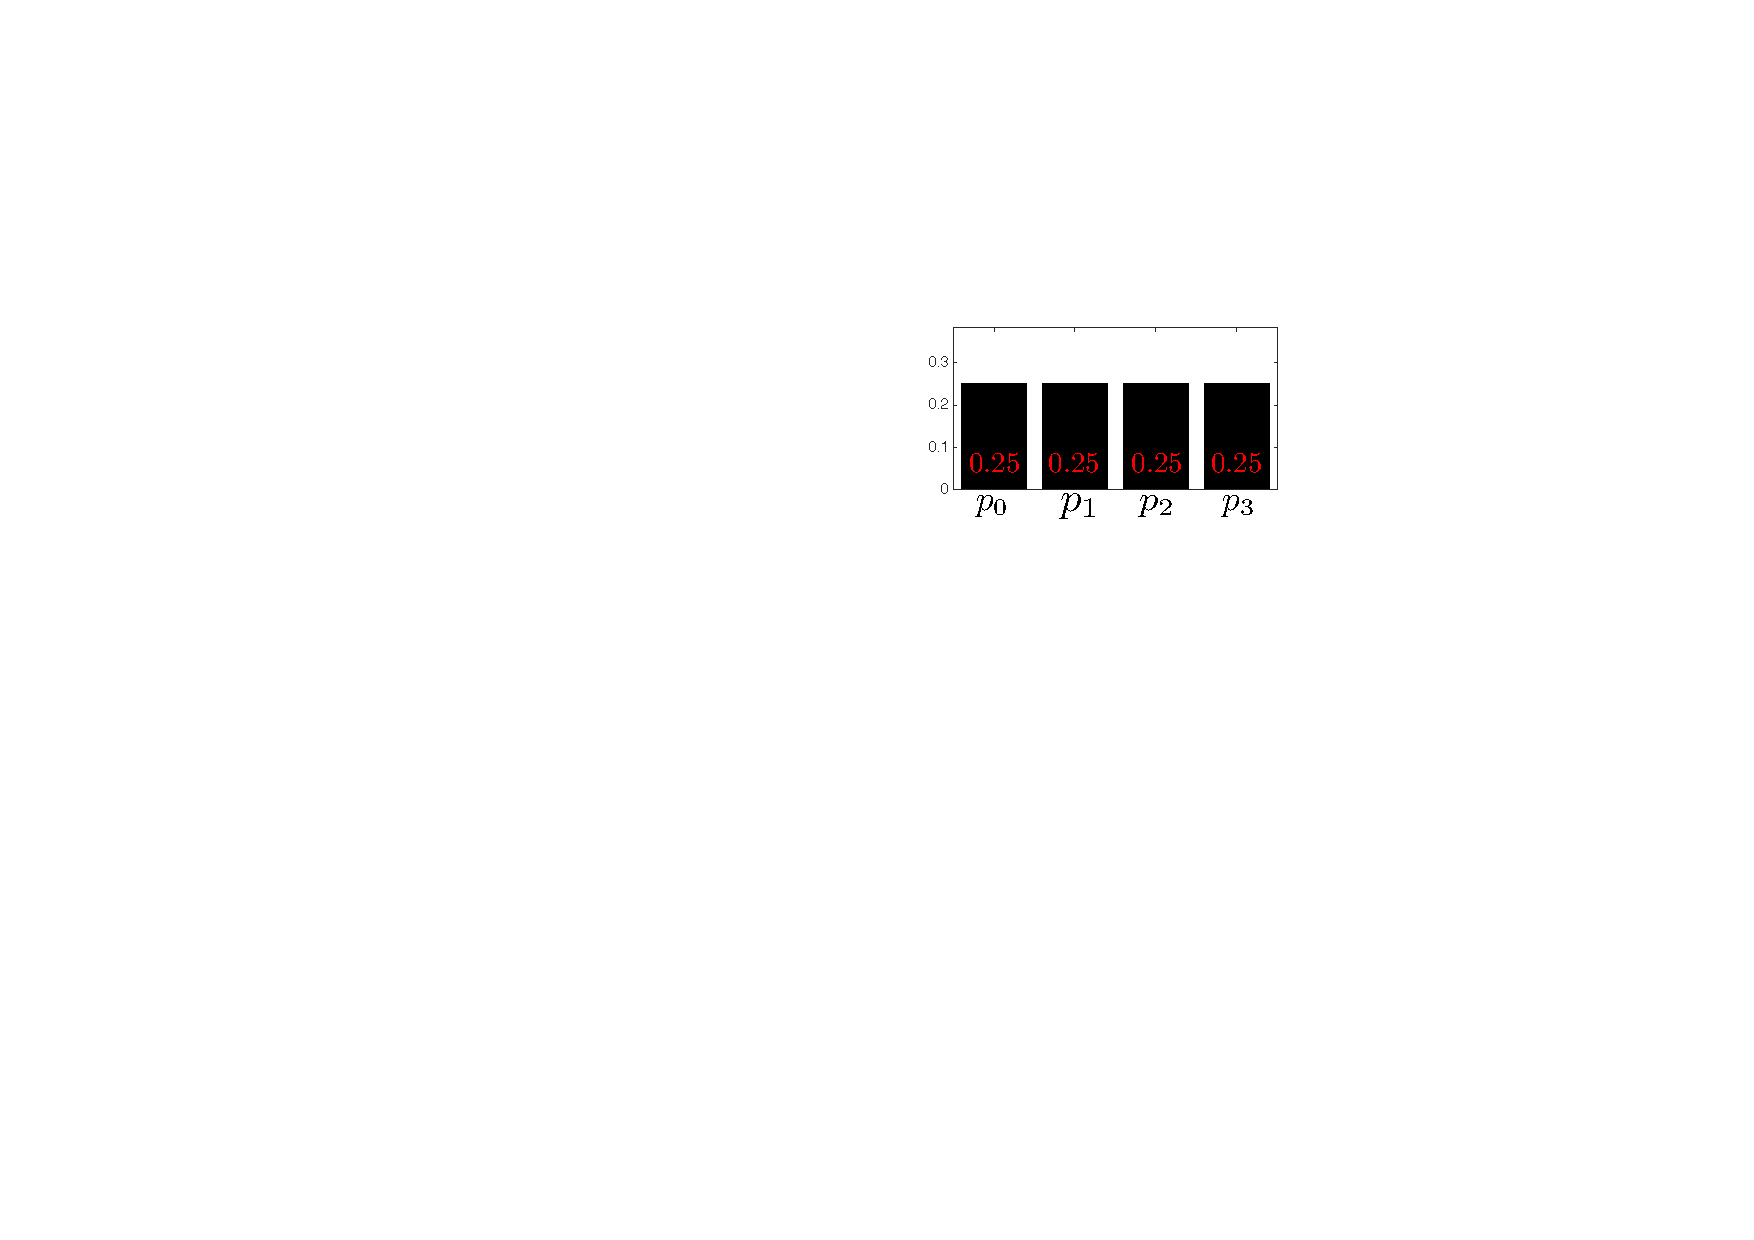
\includegraphics[width=.25\linewidth]{1-shannon/entropie/histo-3}&
\includegraphics[width=.25\linewidth]{1-shannon/entropie/histo-sub}\\
$H(p)=0$ & $H(p)=\log_2(2)=1$ &  $H(p) = 1.62$
}
}{Three examples of probability distributions with corresponding entropies.}{fig-histo-entropy}


\myfigure{
	\image{1-shannon}{.35}{entropy-extrema}
}{%
	Linked extrema for the entropy. %	
}{fig-entropy-extrema}



\begin{lem} One has
\eq{
	0 \leq H(p) \leq \log_2(K).
}
\end{lem}


\begin{proof}
	First one notes that $-x\log_2(x) \geq 0$ for $x \in [0,1]$ (see figure above), so that $H \geq 0$.
	% 
	We consider the following constrained optimization problem
	\eq{
		\max_{p \geq 0} \enscond{ H(p) }{ g(p) = \sum_k p_k =1 }
	}
	see Fig.~\ref{fig-entropy-extrema}.
	%
	First we show that maximizers $p^\star$ are necessarily reached on the interior of the domain, i.e. $p^\star>0$.
	%
	If $p_k^\star=0$ for some $k$, necessarily there exists $\ell \neq k$ such that $p_\ell^\star>0$ (since $p^\star$ cannot be zero), and we study the function 
	$t \geq 0 \mapsto \phi(t) = - ( t \log(t) + (p_\ell^\star-t) \log(p_\ell^\star-t) )$. One shows that it is strictly increasing for $t$ near zero, so that $p^\star$ cannot be a maximum.	
	%
	The function $H$ is smooth on the interior of its domain of definition, so that 
	at an optimum $p^\star>0$, $\nabla H(p^\star)=\la \nabla g(p^\star) = \la (1,\ldots,1)^\top$ for some $\la \in \RR$, so that here $-\log(p_k^\star)-1 = \la$, i.e. $p_k^\star=c$ is constant, and since  $\sum_k p_k^\star=1$, one has $p_k^*=1/K$ and thus $H(p)=\log_2(K)$.
\end{proof}


%%
\paragraph{Shannon theorem.}

%
Assuming that $(p_k)_k$ is the empirical probability of appearance of the symbols $x_k$ in the data to be coded, the average symbol length associated to some code $c$ is 
\eq{
	L(c) \eqdef \sum_k p_k |c_k|. 
}
The goal is to design the best possible $c$ so that $L(c)$ is as small as possible.
%
Shannon theorem of entropic coding, proved bellow, give both lower and upper bound for this question. 

\begin{thm}
	(i) If $c=\text{Leaves}(T)$ for some tree $T$, then 
	\eq{
		L(c) \geq H(p).
	}
	(ii) Conversely, there exists a code $c$ with $c=\text{Leaves}(T)$ such that 
	\eq{
		L(c) \leq H(p)+1.
	}
\end{thm} 

Before proving this theorem, we prove Kraft inequality, which describes the set of prefix codes using an inequality.

\begin{lem}[Kraft inequality]\label{lem-kraft}
	(i) For a code $c$, if there exists a tree $T$ such that $c=\text{Leaves}(T)$ then
	\eql{\label{eq-kraft-ineg}
		\sum_k 2^{-|c_k|} \leq 1.
	}
	(ii) Conversely, if $(\ell_k)_k$ are such that
	\eql{\label{eq-kraft-ineg-2}
		\sum_k 2^{-\ell_k} \leq 1
	}
	then there exists a code $c=\text{Leaves}(T)$ such that $|c_k|=\ell_k$.
\end{lem} 

\begin{proof}
	$\Rightarrow$ We suppose $c=\text{Leaves}(T)$. We denote $m=\max_k |c_k|$ and consider the full binary tree.
	%
	Bellow each $c_k$, one has a sub-tree of height $m-|c_k|$, see Figure~\ref{fig-fourier-wav}, left. This sub-tree has $2^{m-|c_k|}$ leaves. Since all these sub-trees do not overlap, the total number of leaf do not exceed the total number of leaves $2^m$ of the full binary tree, hence
	\eq{
		\sum_k 2^{m-|c_k|} \leq 2^m, 
	}
	hence~\eqref{eq-kraft-ineg}.
	
	\myfigure{
	\image{1-shannon}{.35}{kraft-ineq-1}\quad
	\image{1-shannon}{.45}{kraft-ineq-2}
}{%
	Left: full binary tree obtained by completing the tree associated to the code $(c_1=0, c_2=10, c_3=110, c_4=111)$. 
	%
	Right: packing sub-trees associated to code length to form the left part of the full tree. %	
}{fig-fourier-wav}

	
	$\Leftarrow$ Conversely, we assume~\eqref{eq-kraft-ineg} holds. Without loss of generality, we assume that $|c_1| \geq \ldots \geq |c_K|$. We start by putting a sub-tree of height $2^{m-|c_1|}$. Since the second tree is smaller, one can put it immediately aside, and continue this way, see Figure~\ref{fig-fourier-wav}, right. Since  $\sum_k 2^{m-|c_k|} \leq 2^m$, this ensure that we can stack side-by-side all these sub-tree, and this defines a proper sub-tree of the full binary tree. 
\end{proof}



\begin{proof}[Shannon theorem]
	First, we consider the following optimization problem
	\eql{\label{eq-proof-shannon}
		\umin{ \ell = (\ell_k)_k } \enscond{ f(\ell) \eqdef \sum_k \ell_k p_k }{ g(\ell) \eqdef  \sum_k 2^{-\ell_k} \leq 1 }.
	}
	We fist show that at an optimal $\ell^\star$, the constraint is saturated, i.g. $g(\ell^\star)=1$. Indeed, if $g(\ell^\star)=2^{-u} < 1$, with $u>0$, we define $\ell_k' \eqdef \ell_k^\star-u$, which satisfies $g(\ell') = 1$ and also $f(\ell')=\sum_k (\ell_k-u) p_k < f(\ell^\star)$, which is a contradiction.
	So we can restrict in~\eqref{eq-proof-shannon} the constraint to $g(\ell)=1$ and apply the linked extrema theorem, which shows that necessarily, there exists $\la \in \RR$ with $\nabla f(\ell^\star)=\nabla g(\ell^\star)$, i.e.  $(p_k)_k = -\la \ln(2) (2^{-\ell_k^\star})_k$. Since 
	\eq{
		1 = \sum_k p_k = -\la \ln(2) \sum_k 2^{-\ell_k} = - \la \ln(2) 
	}
	we deduce that $\ell^\star_k = -\log(p_k)$. 
	
	(i) If $c=\text{Leave}(T)$, the by Kraft inequality~\eqref{eq-kraft-ineg}, necessarily $\ell_k=|c_k|$ satisfy the constraints of~\eqref{eq-proof-shannon}, and thus $H(p) = f(\ell^\star) \leq f(\ell) = L(\ell)$.
	
	(ii) We define $\ell_k \eqdef \lceil -\log_2(p_k) \rceil \in \NN^*$. Then $\sum_k 2^{-\ell_k} \leq \sum_k 2^{\log_2(p_k)} = 1$, so that these lengths satisfy~\eqref{eq-kraft-ineg-2}. Thanks to Proposition~\ref{lem-kraft} (ii), there thus exists a prefix code $c$ with $|c_k|=\lceil -\log_2(p_k) \rceil$. Furthermore
	\eq{
		L(c) = \sum_k p_k \lceil -\log_2(p_k) \rceil \leq \sum_k p_k ( -\log_2(p_k) +1) = H(p)+1.
	}
\end{proof}

Note that this proof is constructing, i.e. it gives an algorithm that construct an almost optimal $c$, and this code is often called the Shannon-Fano code. It is usually a good code, although it is not necessarily the optimal code with the smallest $L(c)$. Such an optimal code can easily be computed in almost linear time (only sorting of the probability is needed, so it is $K(\log(K))$) by Huffman's dynamic programming algorithm (invented in 1952). The proof of correctness of this algorithm is however a bit tedious. Figure~\ref{fig-huff-code} shows an example of application of this algorithm.


\texttt{Associated code: coding/test\_text.m}

In practice, such an entropic coding, although optimal, is not very efficient when one of the symbol has a large probability $p_k$. This is because then $2^{-p_k} \ll 1$ but one cannot allocate a fractional number of bit. This is why $L(c)$ can be as large as $H(p)+1$. A simple workaround is to artificially increase the size of the alphabet from $K$ to $K^r$ by grouping together sets of $r$ consecutive symbols, and thus reducing the gap to $H(p)+1/r$. Constructing the code and coding however becomes very slow for large $r$. The standard way to achieve this without explicitly doing the grouping is by using arithmetic coding, invented in 1976, which using interval arithmetic to allocate fractional number of bits and leveraging the fact that one usually code large sequence, thus approaching to arbitrary precision Shannon bound $H(p)$ as the length of the data increases.


\myfigure{
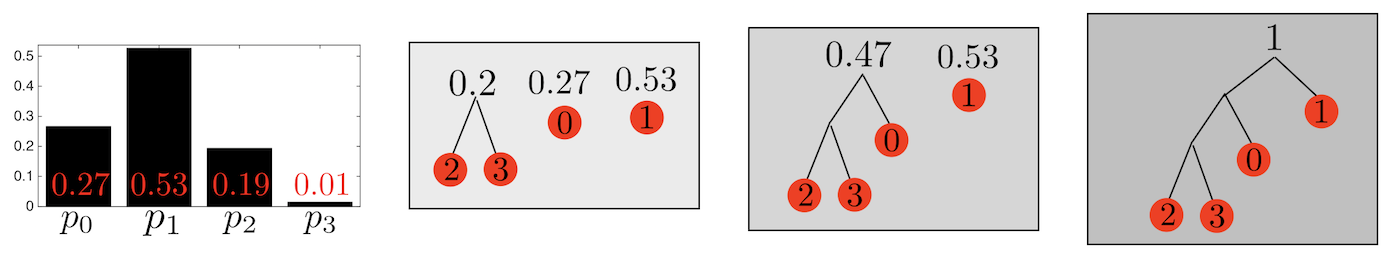
\includegraphics[width=.8\linewidth]{1-shannon/huff-code}
}{Huffman coding algorithm in action.}{fig-huff-code}

Note that while we give some statistical and probabilistic interpretation of entropy (measure of uncertainty) and of Shannon theorem, this theory is fully deterministic and give a bound for the actual length $N L(c)$ of coding some sequence of length $N$ if the probability $p$ are the empirical probability of the sequence.

If one choose a different probability $q$ and use it to code the sequence, one necessarily obtain a worse average coding length, and this is reflected by the positivity of the so-called relative entropy (beware that it is a convex function while the entropy is concave), which is often called the Kulback-Leibler divergence
\eq{
	\text{KL}(p|q) = -\sum_k p_k \log q_k - H(p)   = \sum_k p_k \log \frac{p_k}{q_k} \geq 0.
}
This KL divergence is similar to a distance in the sense that $\text{KL}(p|q)=0$ if and only if $p=q$ (note however that KL is not symmetric and does not satisfies the triangular inequality). It also has the remarkable property that it is jointly convex in $(p,q)$. It is of paramount importance to compare probability distributions and measures, and form the basis of the fields of information theory and information geometry. 


%%
\paragraph{Doing better.}

One can wonder if it is possible to go bellow the entropy bound. By the virtue of Shannon theorem, it is not possible if only can only code in sequential order the symbols themselves. From a statistical perspective, it is as if the symbols where considered to be independent. If there is some redundancy in the sequence of symbol (for instance if they are discretization of a smooth function, so that to consecutive symbols are likely to be equal), it is possible to re-transform (in a bijective way) the sequence to make them ``more independent''. A simple illustration of this idea is given in Figure~\ref{fig-codage-differences}, where one computes successive difference of a 1D sequence of symbols (beware to also retain the initial symbol to be able to do the decoding.

\myfigure{
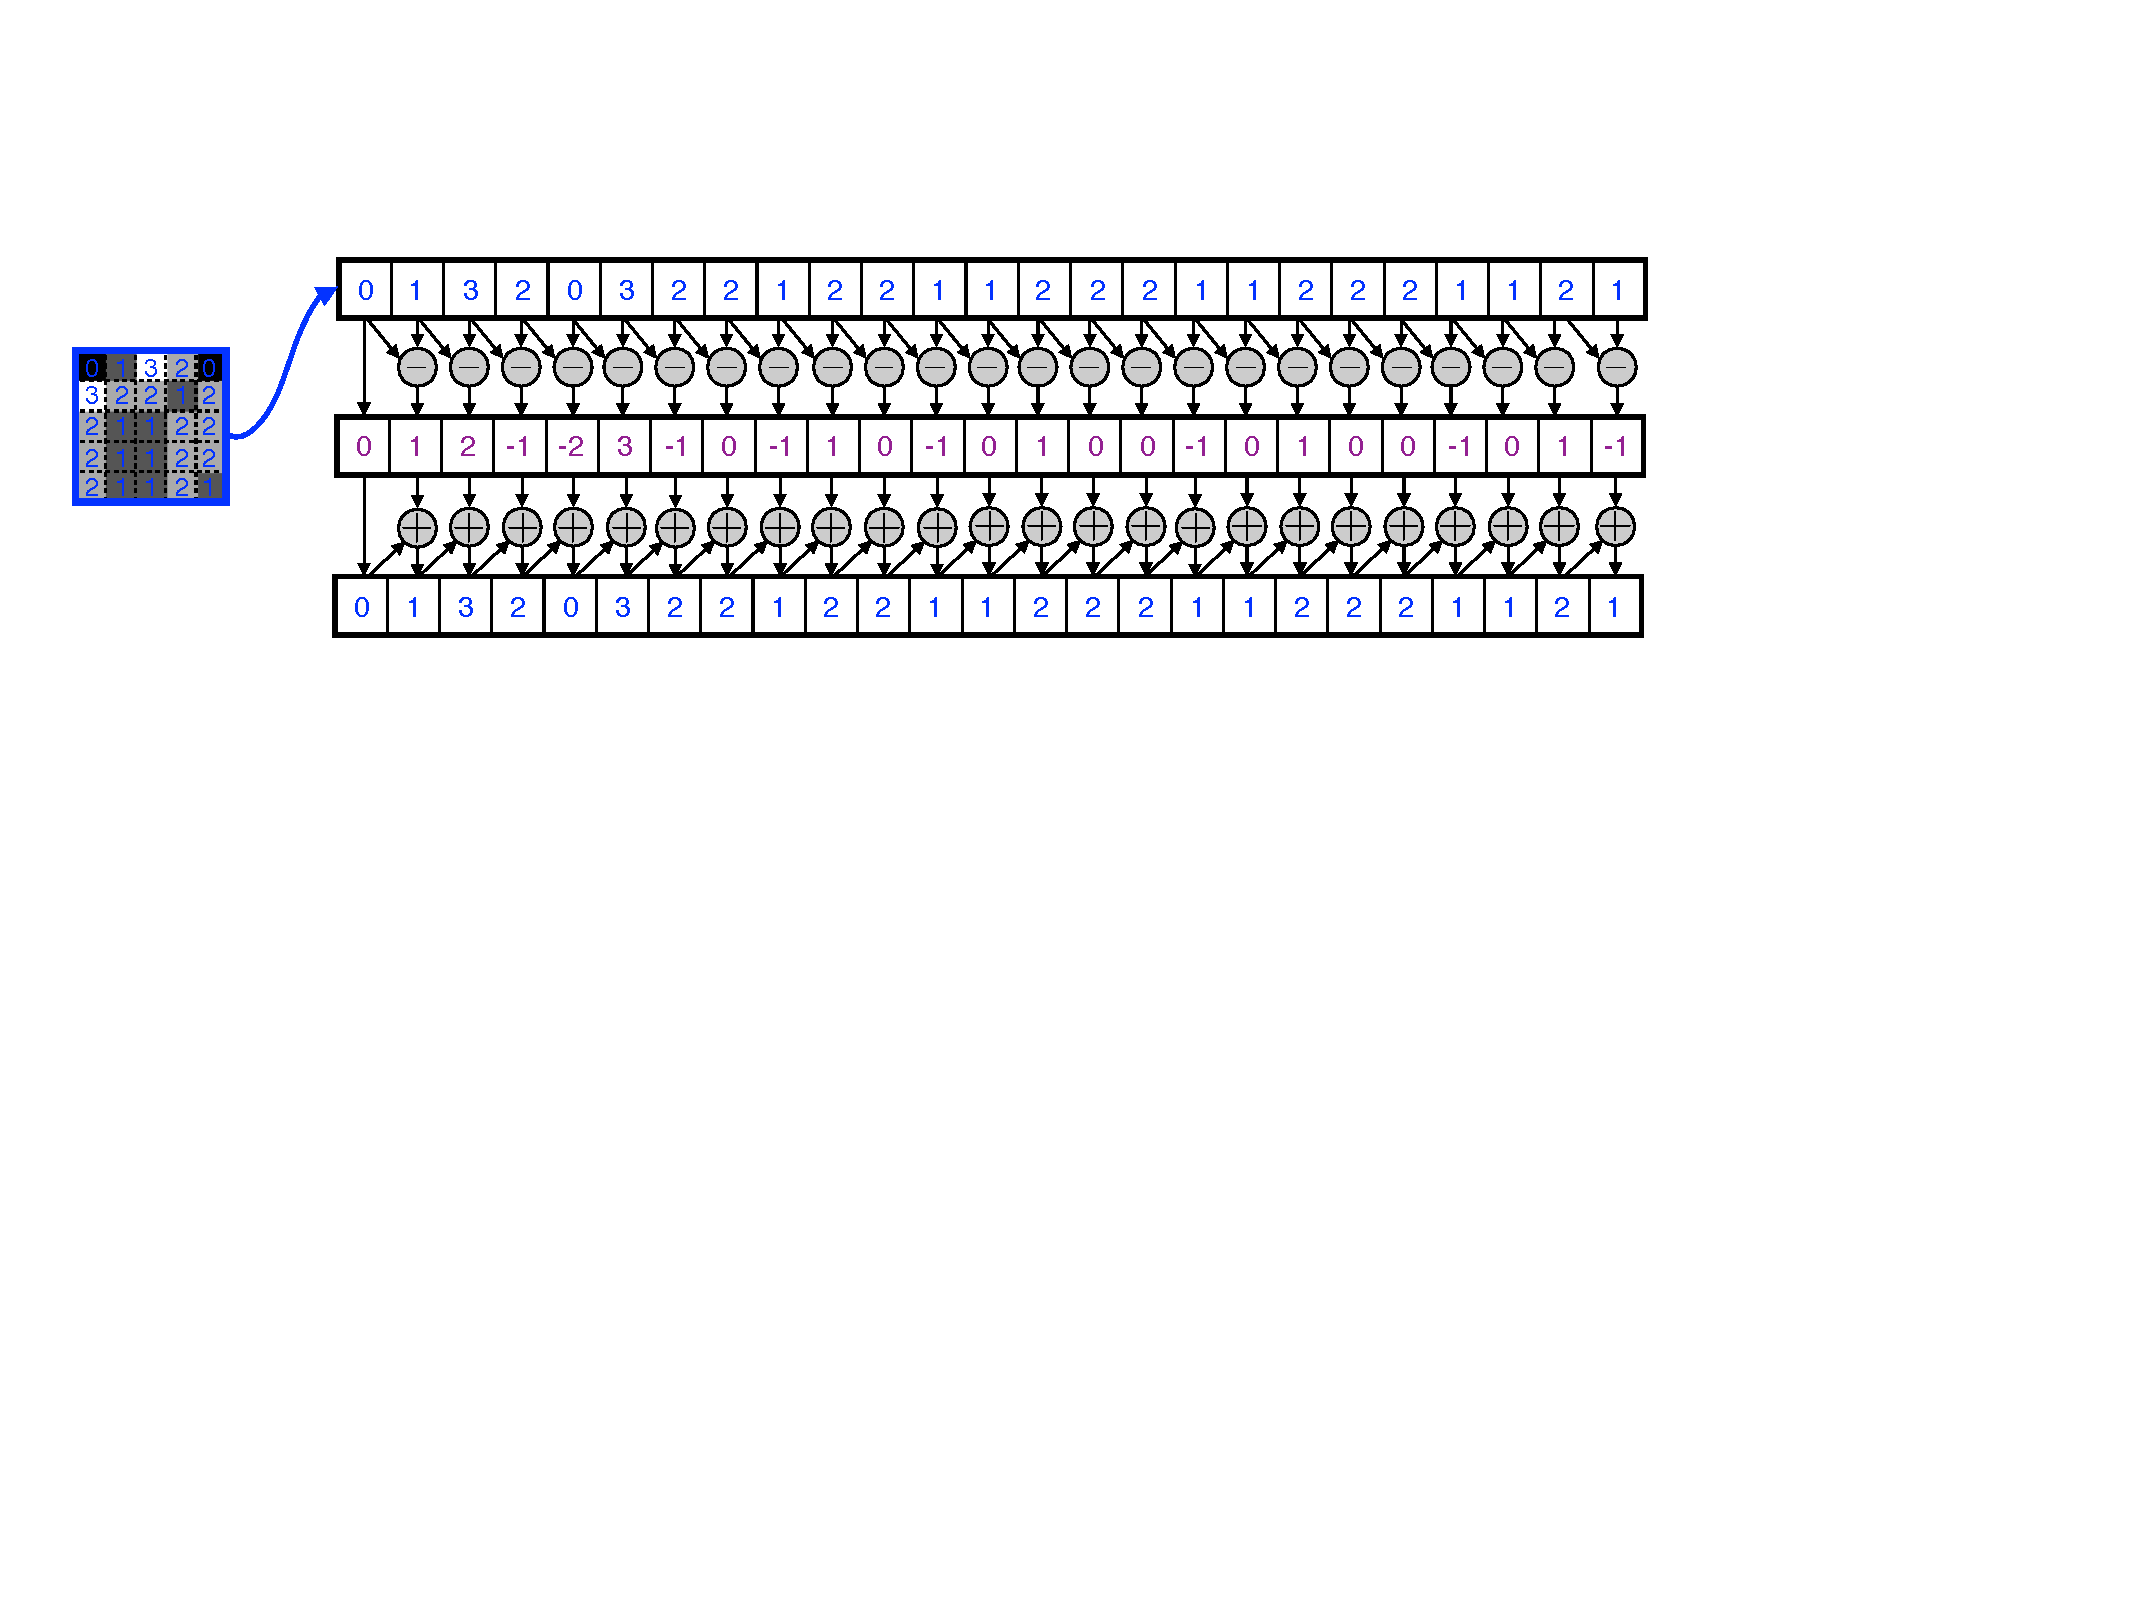
\includegraphics[width=.8\linewidth]{1-shannon/differences/differences}
%
\tabtrois{
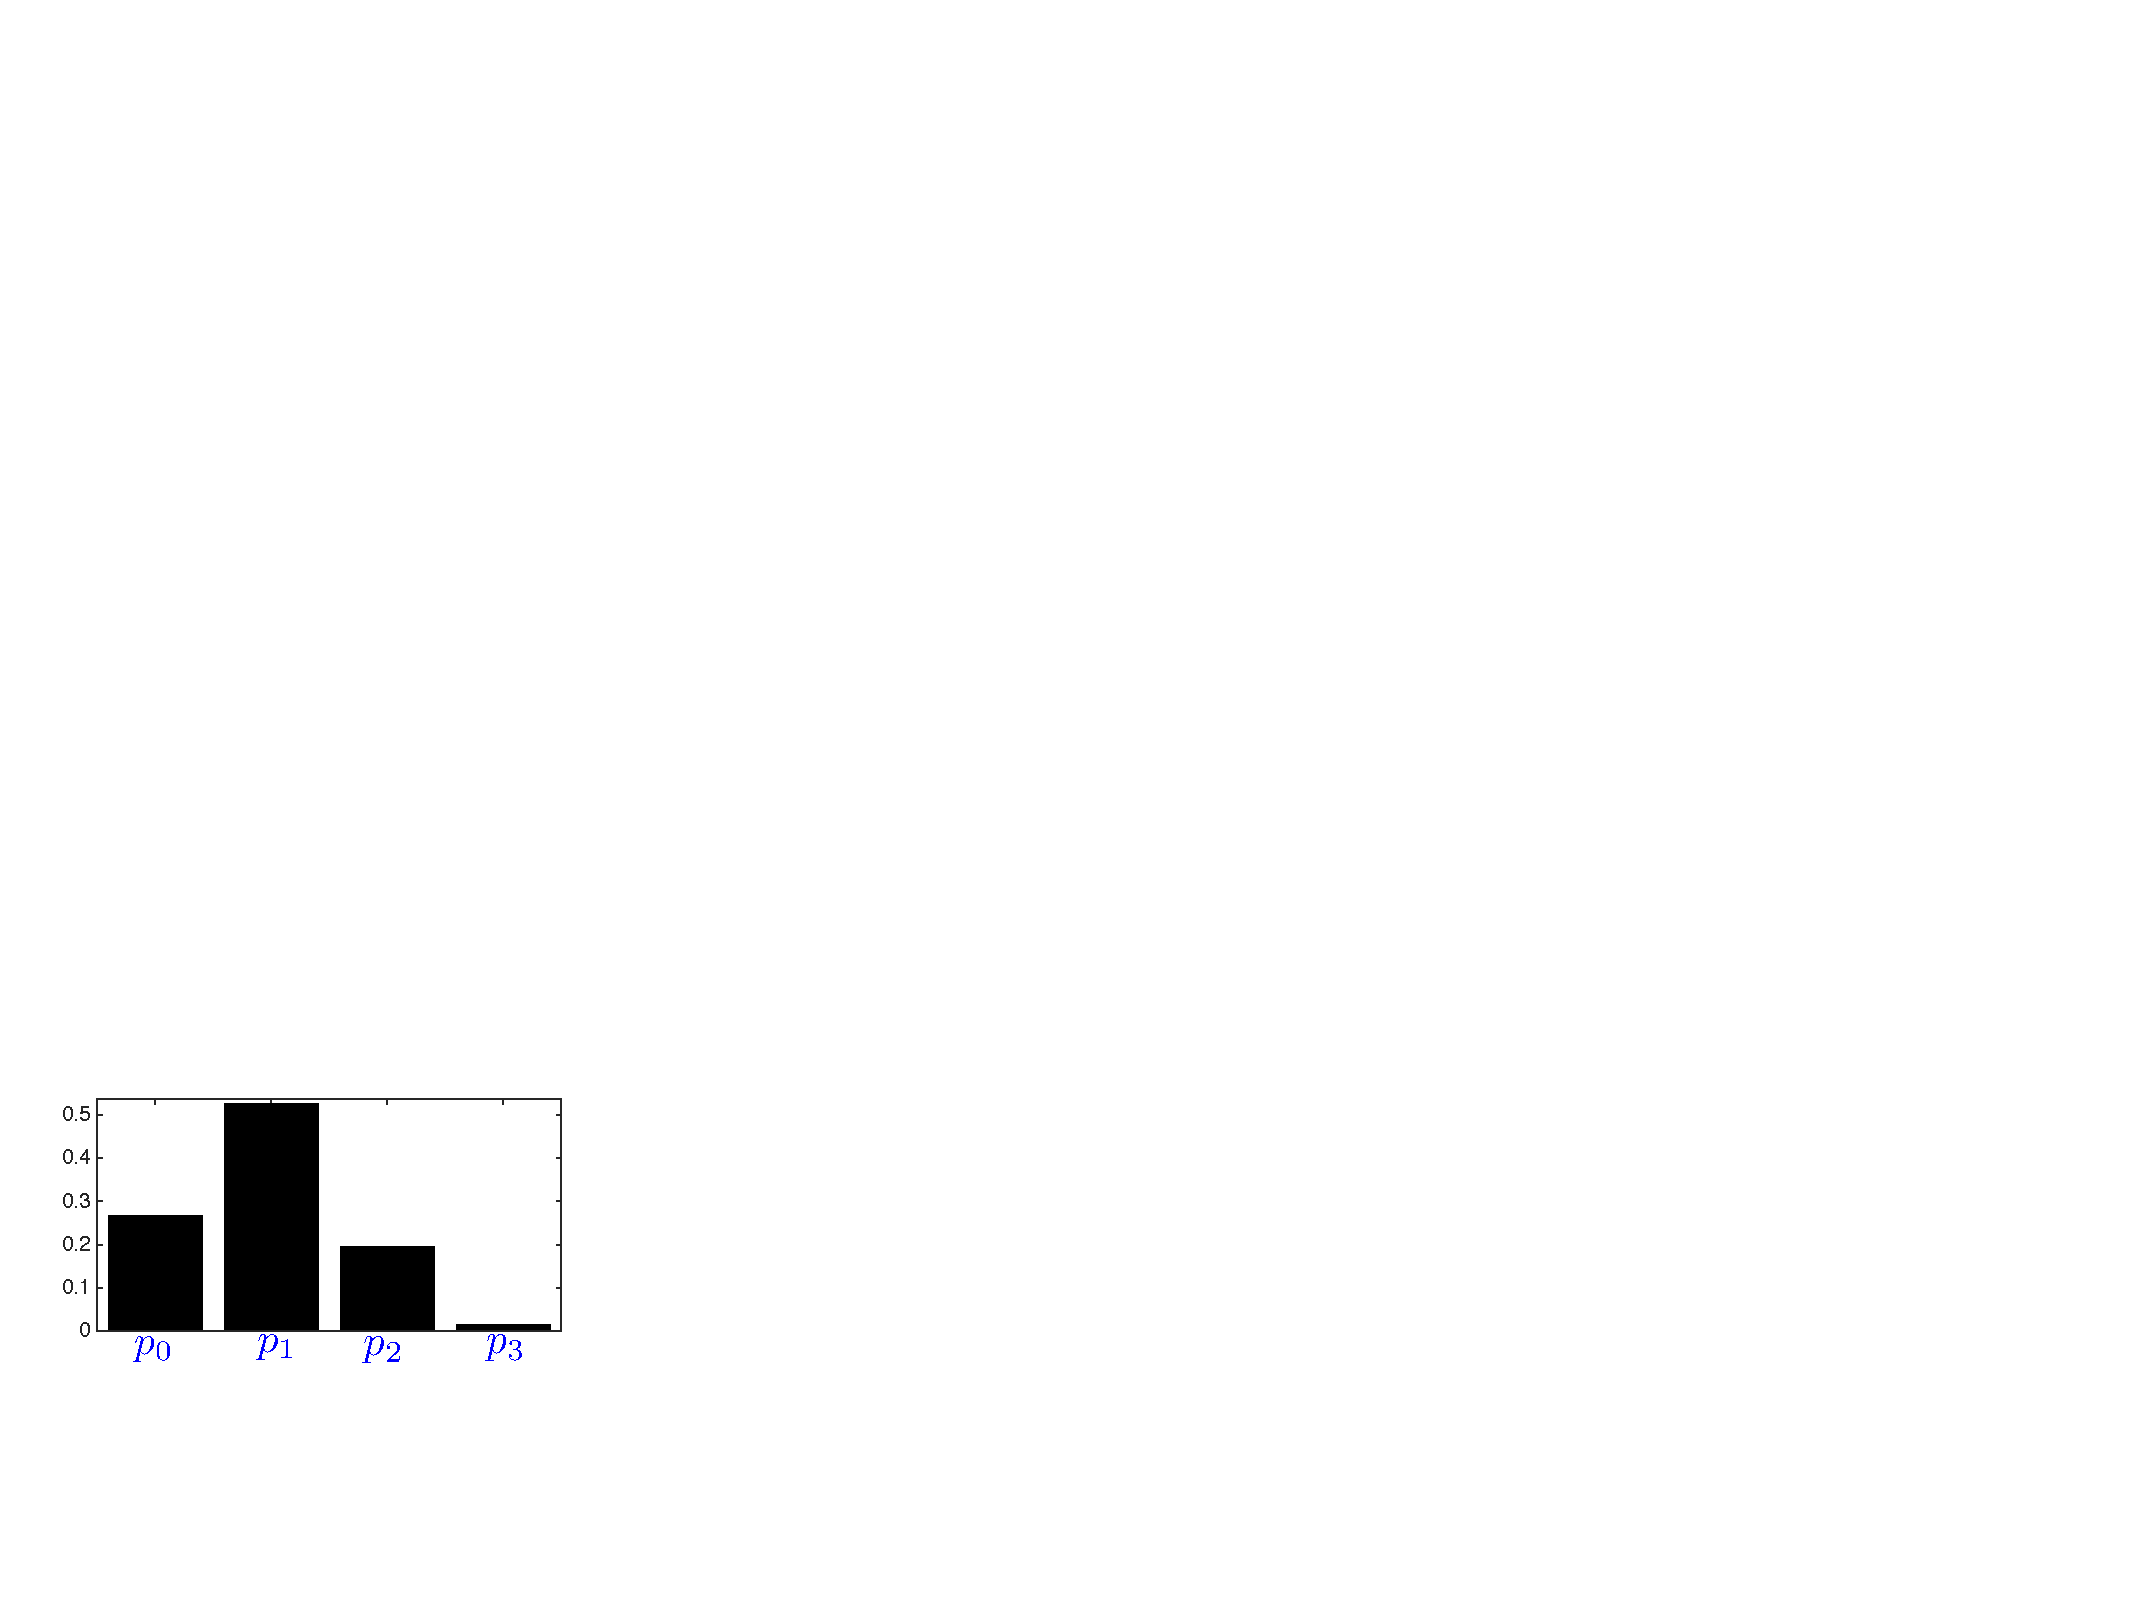
\includegraphics[width=.25\linewidth]{1-shannon/differences/histo-pix}&
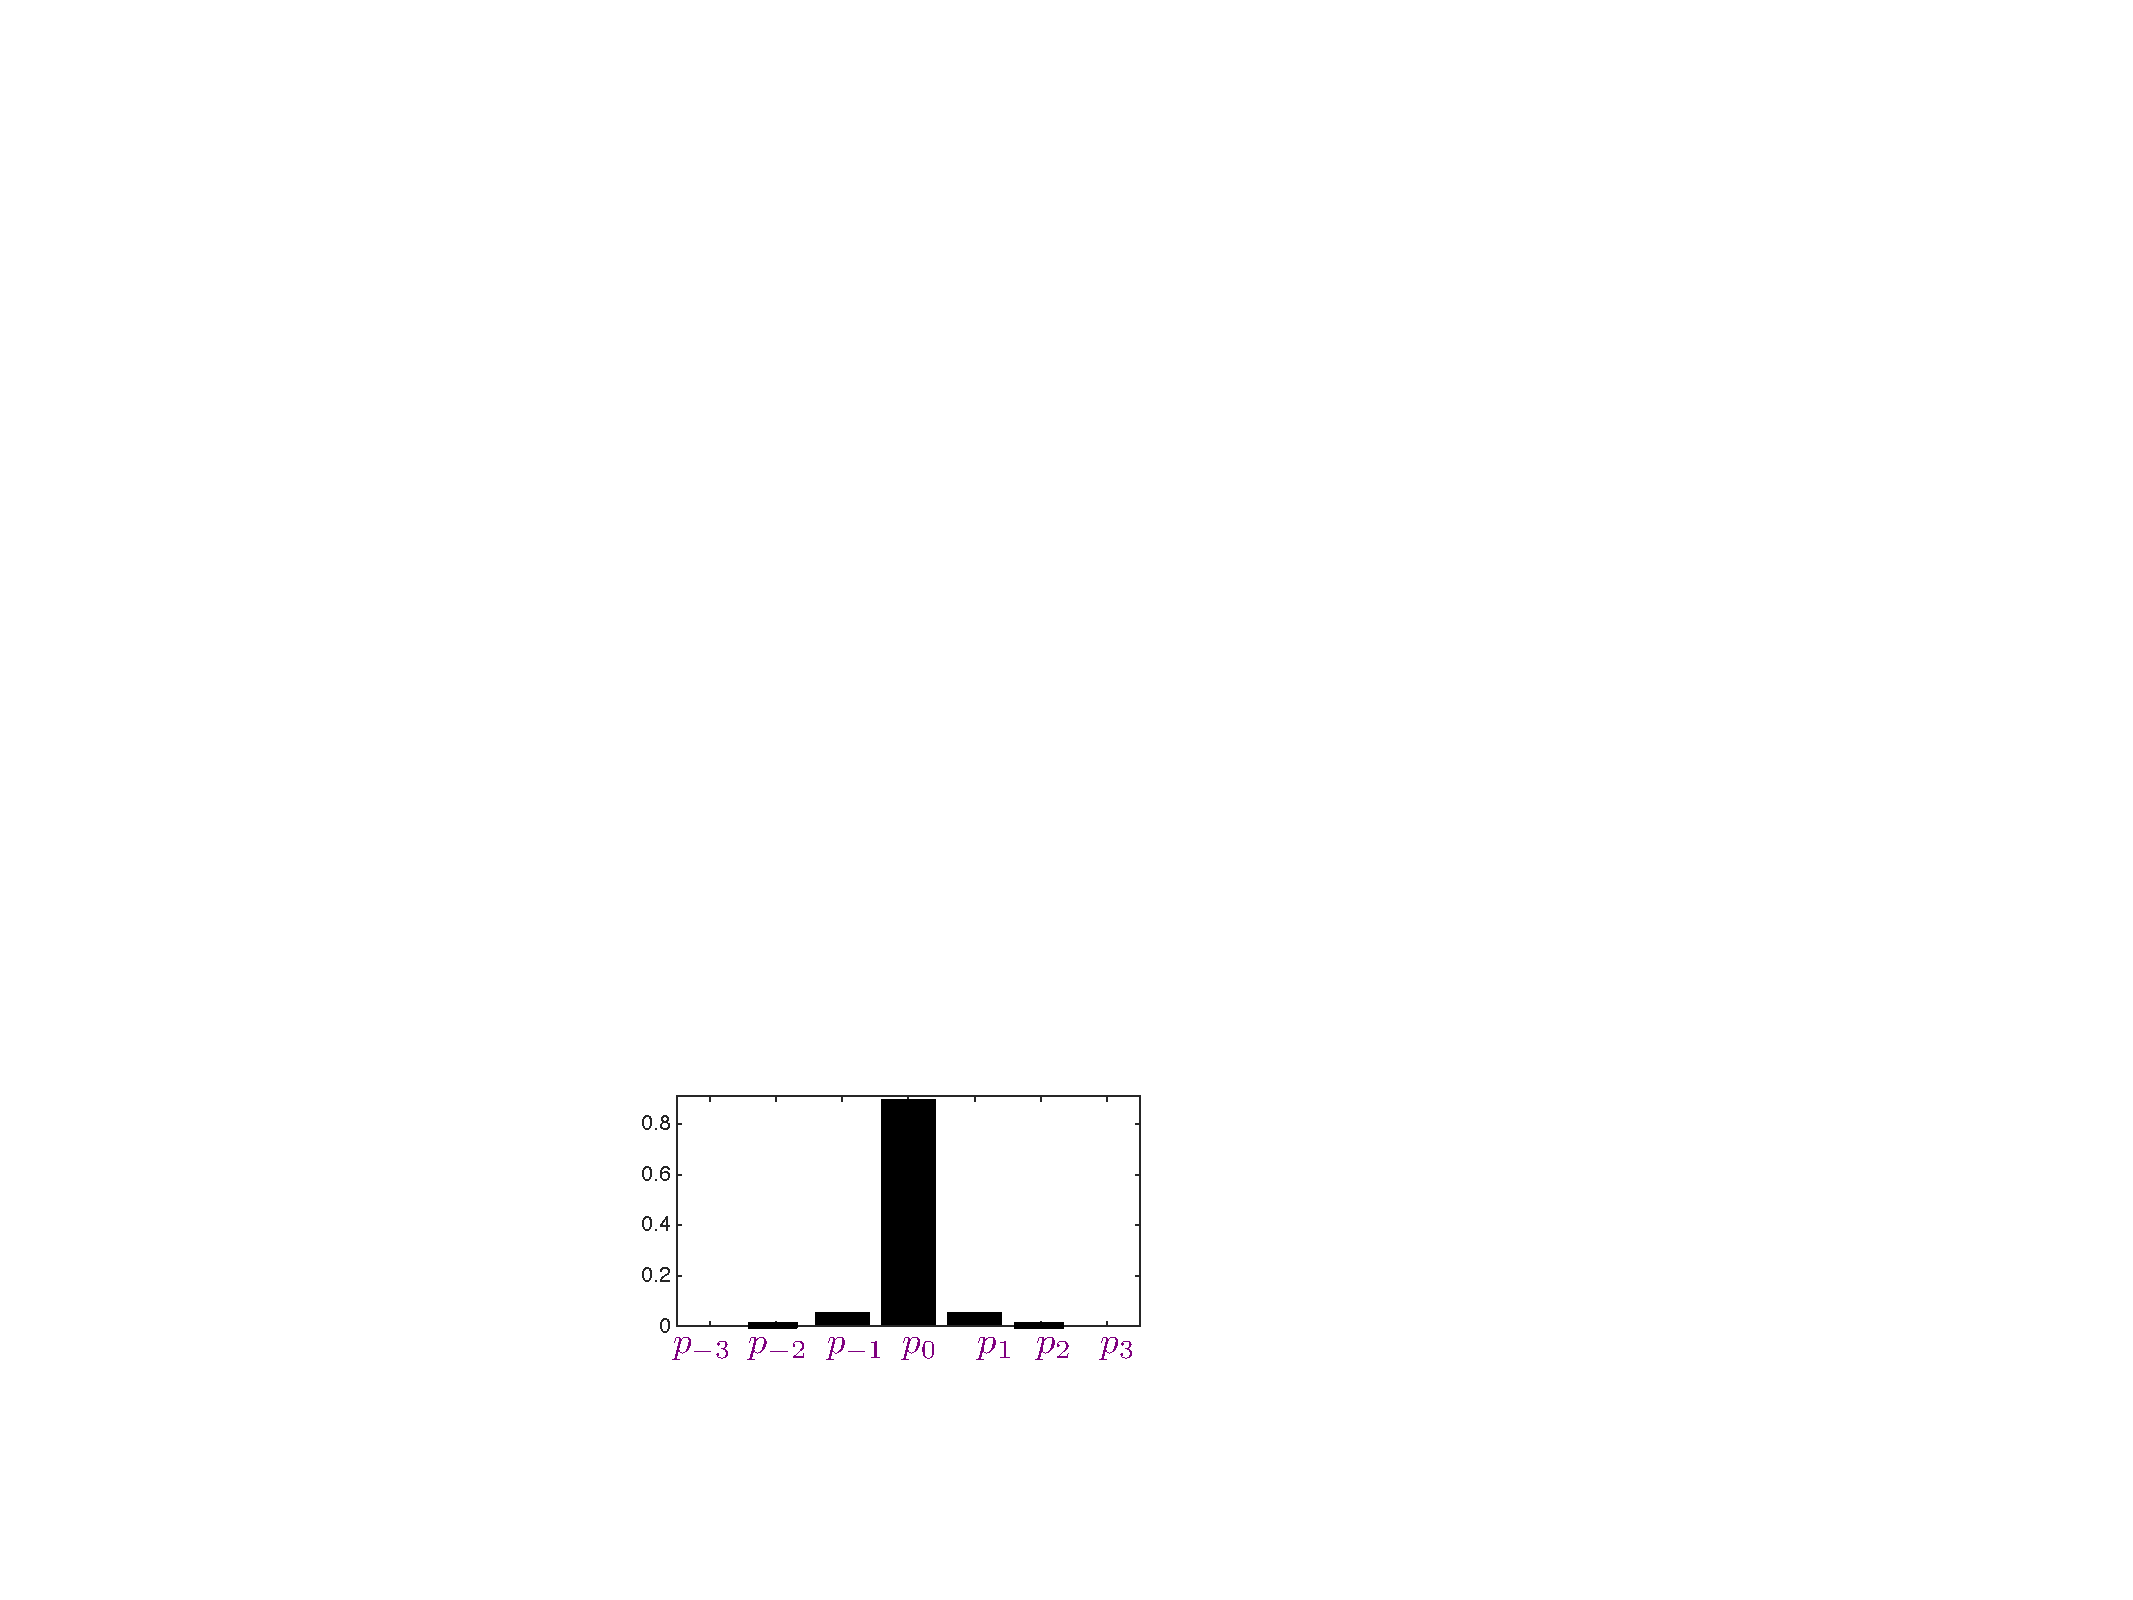
\includegraphics[width=.25\linewidth]{1-shannon/differences/histo-diff}&
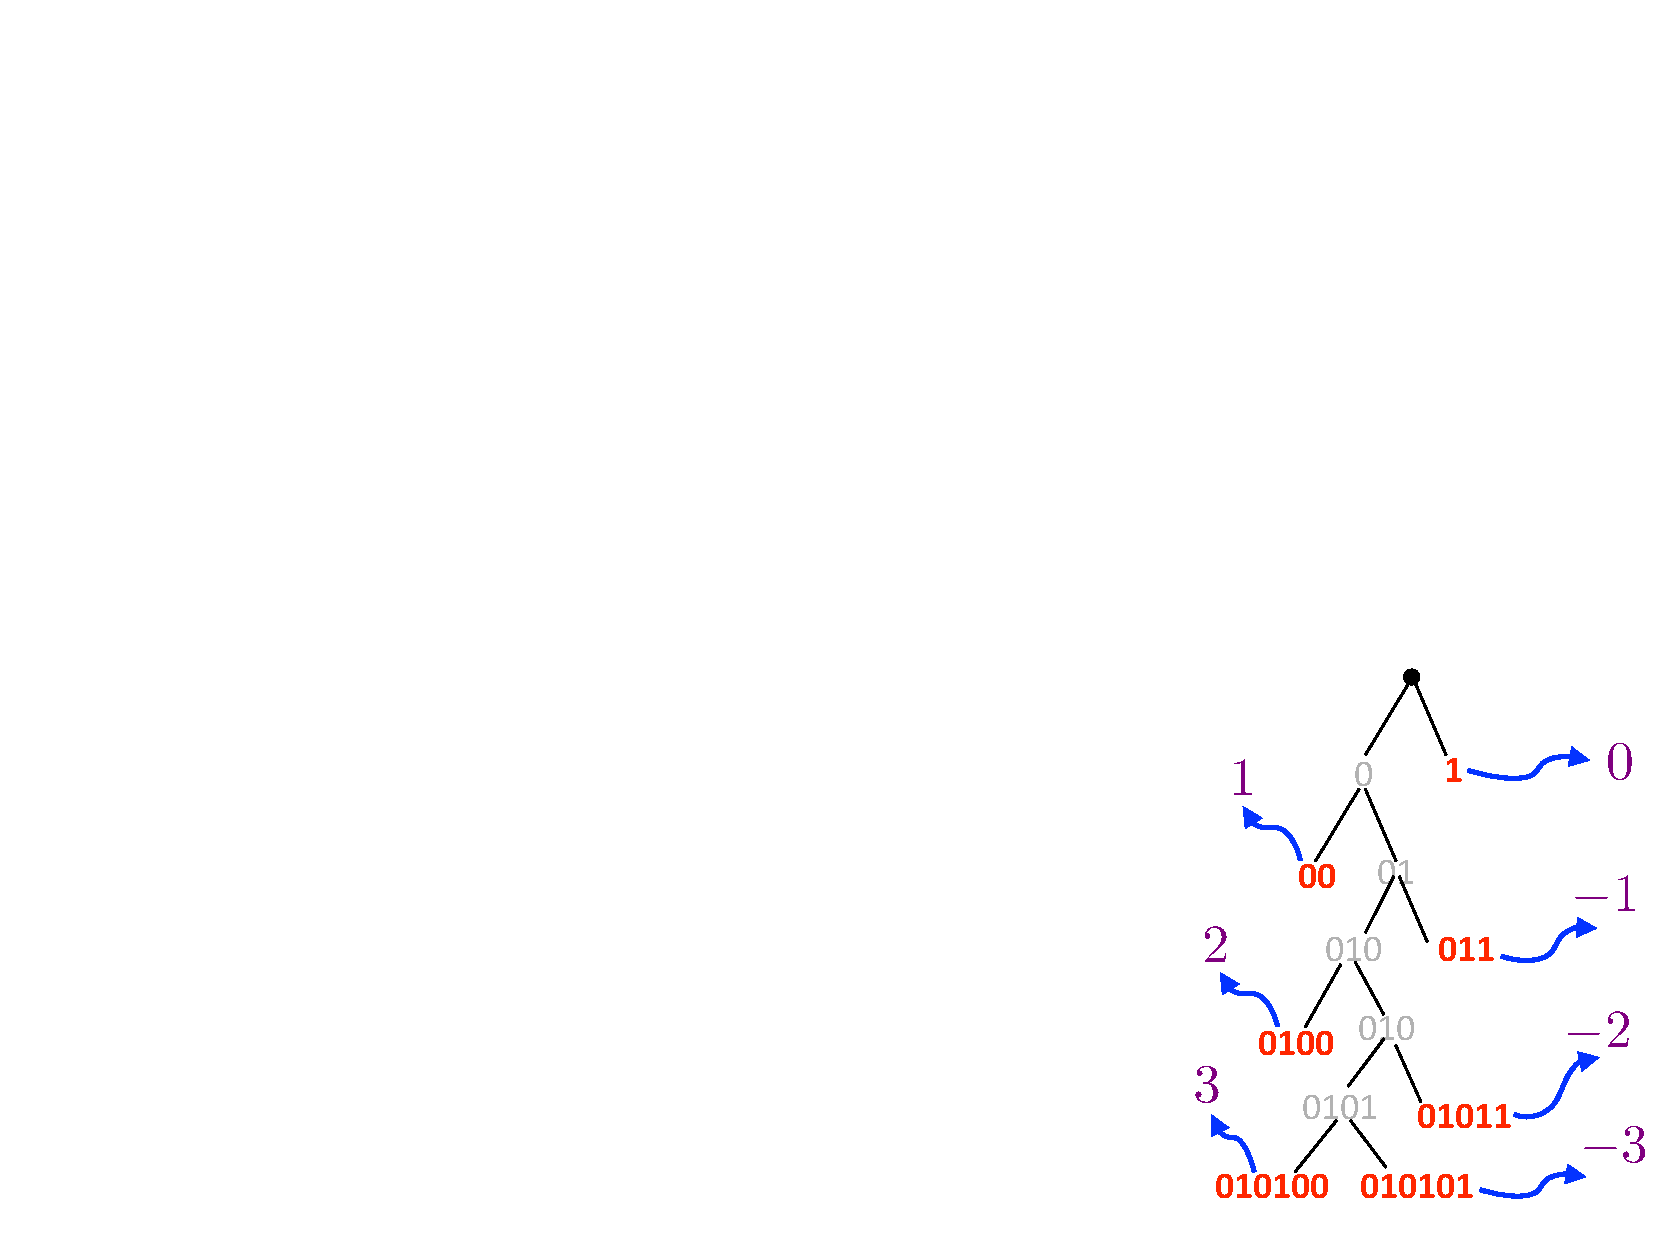
\includegraphics[width=.2\linewidth]{1-shannon/differences/arbre-difference}\\
$H(p) \approx 1.54, L(c) \approx 1.67 $ & $H(p) \approx 0.61, L(c) \approx 1.16 $ & Coding Tree
}
}{Top: retransformation by successive differences.
%
Bottom: comparison of histograms of pixel values and differences, and a code tree for these differences.
%
}{fig-codage-differences}

Another, more systematic way to leverage such temporal redundancy is by performing run-length-coding, which operate by grouping together sequence of similar symbols and thus coding first a symbol and then the length of the associated group (which is coded entropically). If the sequence is generated by a Markov chain, this method can be shown to asymptotically reach the Shannon bound where now the entropy is the entropy associated to the distribution of the Markov chain on infinite sequences (which can be computed as the limit of the entropy for finite sequences).



